Que faire si nous avons des formules trigonométriques impliquant deux variables, ou plus?
Par exemple,
pour
$(\alpha ; \beta) \in \big( \RRsp \big)^2$ tel que $0 < \alpha + \beta < \frac{\pi}{2}$,
le dessin suivant nous donne
$\cos(\alpha + \beta) = \cos \alpha \cos \beta - \sin \alpha \sin \beta$
et
$\sin(\alpha + \beta) = \cos \alpha \sin \beta + \sin \alpha \cos \beta$. 

\begin{center}
	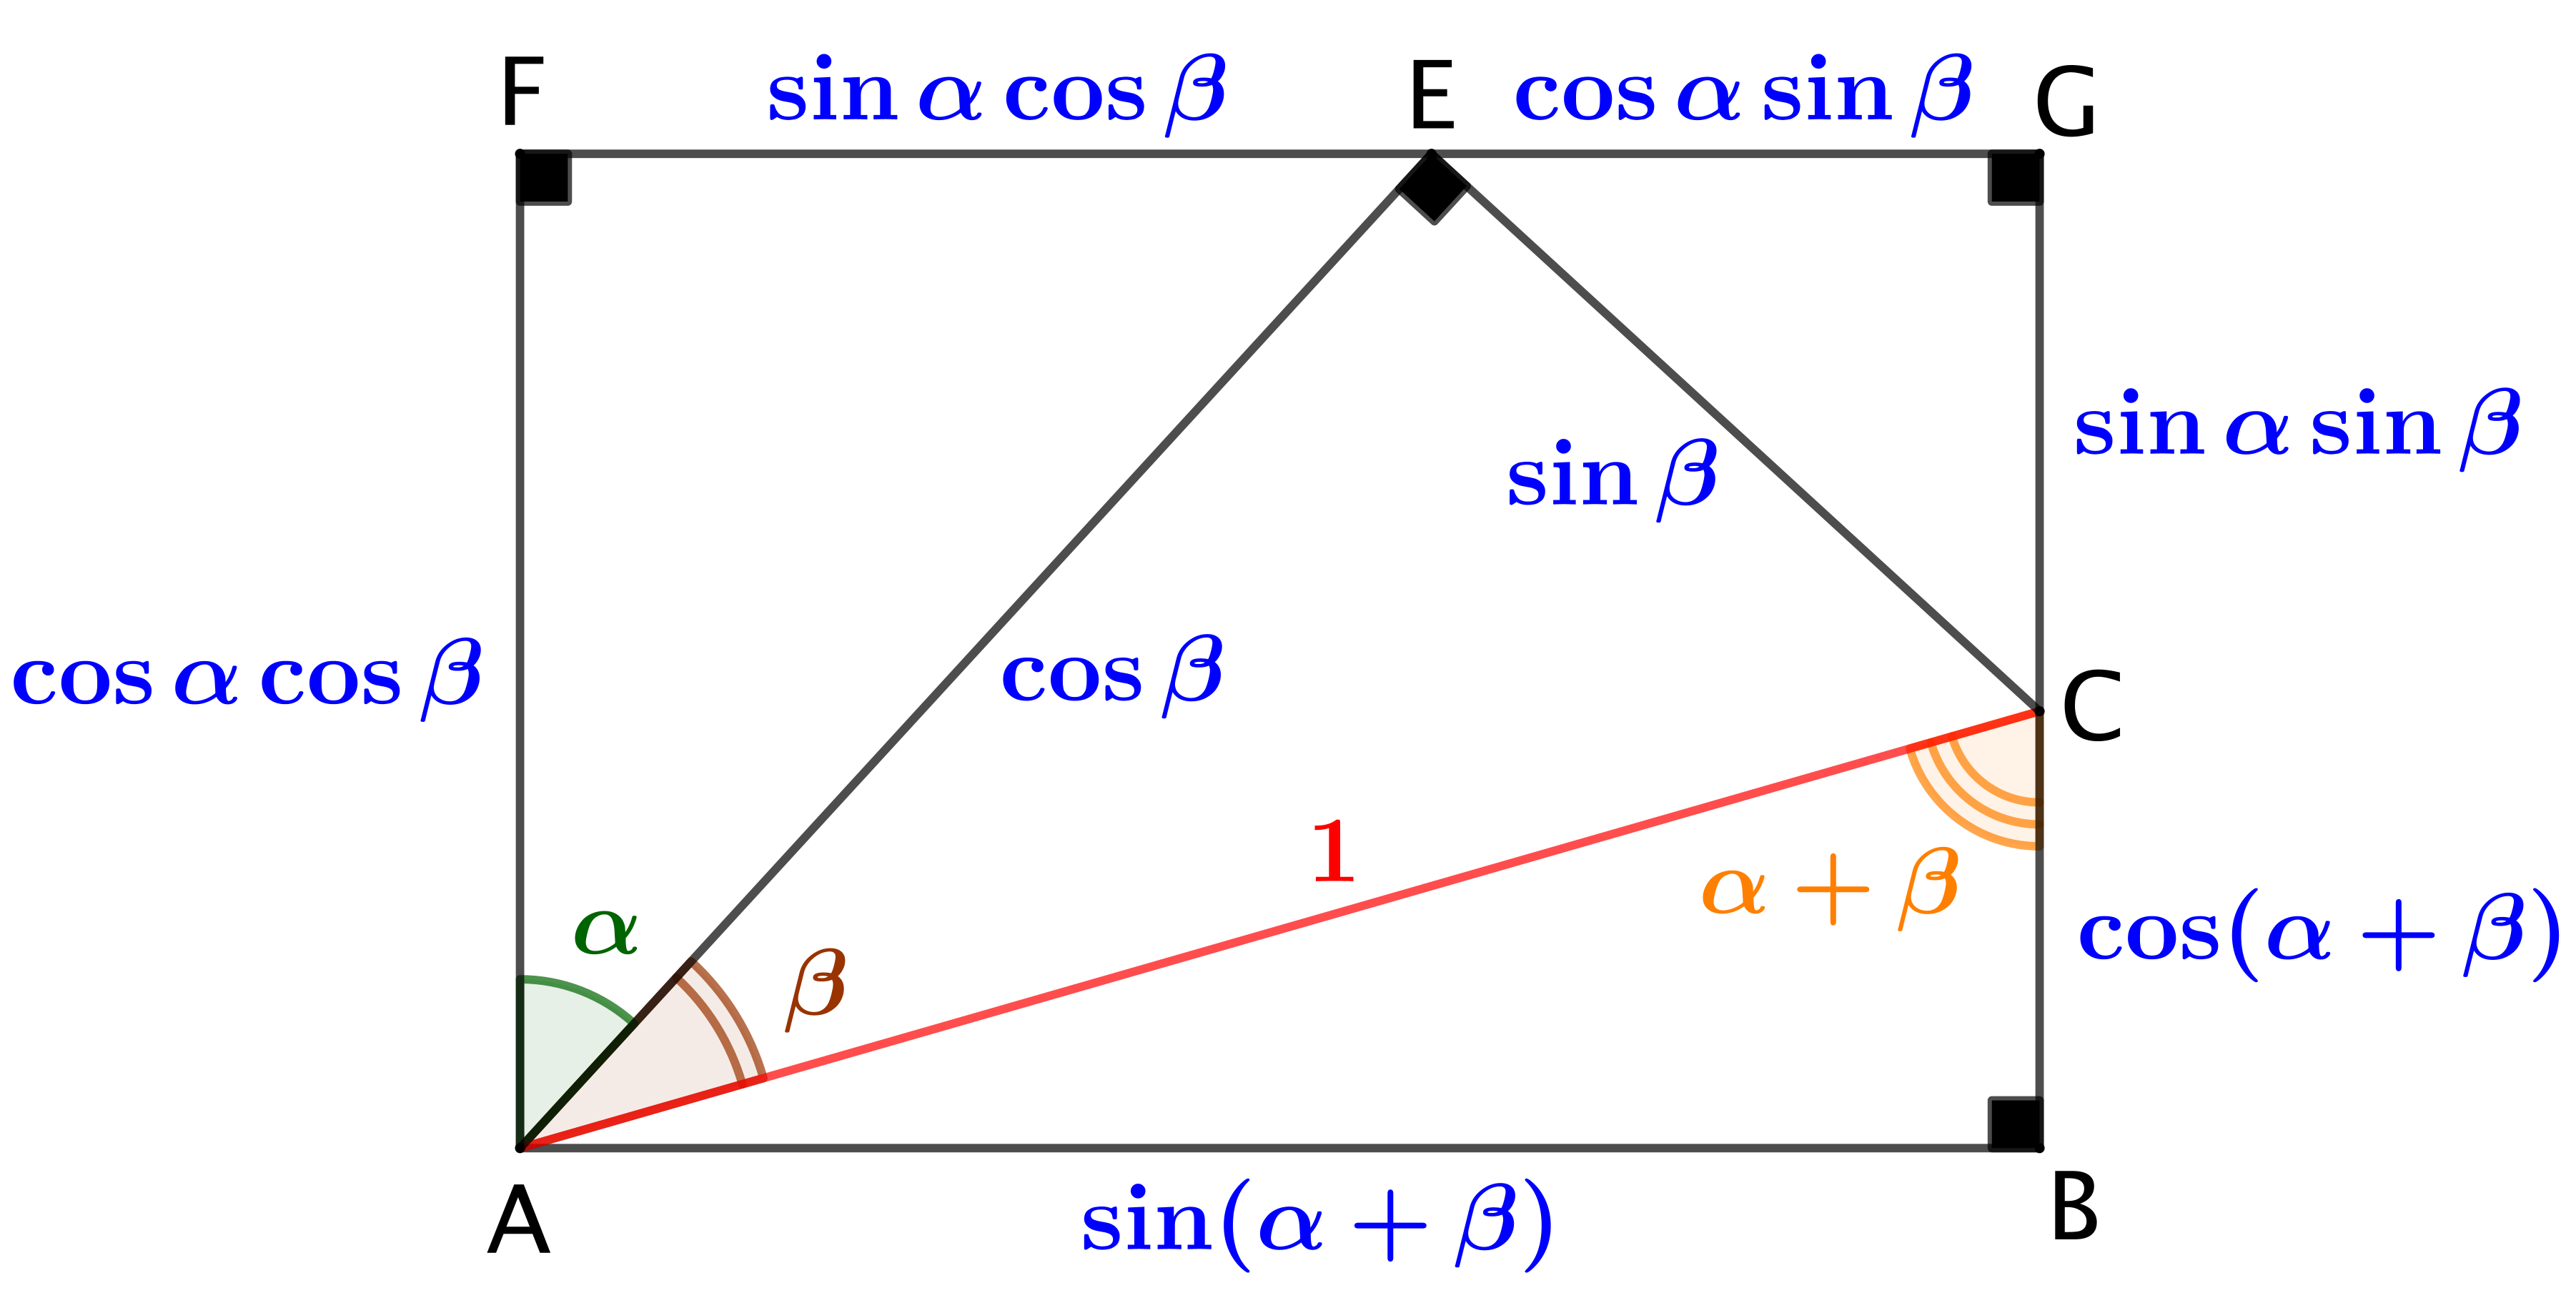
\includegraphics[scale=.7]{two-var-trig-formulas.png}
\end{center}

Le fait \ref{multi-isolated-zero} ci-dessous, qui généralise le fait \ref{isolated-zero}, implique la validité des formules trigonométriques précédentes sur $\CC^2$ tout entier en faisant les choix ci-après.%
\footnote{
    L'ouvert de nullité est l'intérieur d'un triangle.
}
Nous voilà sauvés!
%
\begin{itemize}[label=\small\textbullet]
	\item $f_1(\alpha ; \beta) = \cos(\alpha + \beta) - \cos \alpha \cos \beta + \sin \alpha \sin \beta$

	\item $f_2(\alpha ; \beta) = \sin(\alpha + \beta) - \cos \alpha \sin \beta - \sin \alpha \cos \beta$
\end{itemize}


% ----------- %


\begin{defi}
    Soit $n \in \NNs$.
    Une fonction $f: \CC^n \rightarrow \CC$ sera dite \focus{séparablement analytique} sur $\CC^n$,
    si $\forall i \in \ZintervalO{1}{n}$, 
	la fonction $f_i: z \mapsto f(z_1 ; ... ; z_{i-1} ; z ; z_{i+1} ; ... ; z_n)$ est analytique sur $\CC$.%
	\footnote{
		Avec des abus de notations évidents.
	}
\end{defi}


\begin{fact} \label{multi-isolated-zero}
    Soit $f: \CC^n \rightarrow \CC$ une fonction séparablement analytique, où $n \in \NNs$.
	Si $f$ s'annule sur un ouvert non vide de $\CC^n$, alors $f$ s'annule sur $\CC^n$ tout entier. 
\end{fact}


\begin{proof}
	Raisonnons par récurrence sur $n \in \NNs$ pour démontrer la validité de la propriété $\setproba{P}(n)$ définie par
	\emph{\og 
		Pour toute fonction séparablement analytique $f: \CC^n \rightarrow \CC$,
		si $f$ s'annule sur un ouvert non vide de $\CC^n$,
		alors $f$ s'annule sur $\CC^n$ tout entier. 
	\fg}\kern2pt.
	%
	\begin{itemize}[label=\small\textbullet]
		\item \textbf{Cas de base.}
		%
		$\setproba{P}(1)$ découle directement du fait \ref{isolated-zero}.


		\item \textbf{Hérédité.}
		%
		Supposons $\setproba{P}(n)$ valide pour un naturel $n$ quelconque.
		Soit $f$ une fonction séparablement analytique à $(n + 1)$ variables vérifiant les conditions de la propriété $\setproba{P}(n + 1)$. Notons $\Omega$ l'ouvert sur lequel $f$ est nulle.
		%
		Quitte à réduire $\Omega$, on peut supposer que
		$\Omega = \dprod_{i=1}^{n+1} \CdiscO{\alpha_i}{r}$
		avec $r > 0$ et les $\alpha_i$ des complexes fixés.
		%
		\begin{enumerate}
		    \item Pour $\omega \in \CdiscO{\alpha_{n+1}}{r}$ fixé quelconque,
		    posons $f_\omega(z_1 ; ... ; z_n) = f(z_1 ; ... ; z_n ; \omega)$.
		    Comme $f_\omega$ vérifie les conditions de la propriété $\setproba{P}(n)$, par hypothèse de récurrence, nous avons
		    $f_\omega(z_1 ; ... ; z_n) = 0$, 
		    soit $f(z_1 ; ... ; z_n ; \omega) = 0$,
		    pour $(z_1 ; ... ; z_n) \in \CC^n$.


		    \item Fixons ensuite $z_1$ , ... , $z_n$ des complexes quelconques, et posons $\ell(z) = f(z_1 ; ... ; z_n ; z)$.
		    Le point précédent montre que $\ell$ vérifie $\setproba{P}(1)$, ceci impliquant
		    $\ell(z) = 0$,
		    soit $f(z_1 ; ... ; z_n ; z) = 0$,
		    pour tout complexe $z$, d'après le cas de base.


		    \item Finalement, $f(z_1 ; ... ; z_n ; z) = 0$ pour tous complexes $z_1$ , ... , $z_n$ et $z$.
		    Autrement dit, nous avons déduit la validité de $\setproba{P}(n+1)$ à partir de celle de $\setproba{P}(n)$.
		\end{enumerate}
		
		
		\item \textbf{Conclusion.}
		%
		Par récurrence sur $n \in \NNs$, la propriété $\setproba{P}(n)$ est vraie pour tout naturel non nul $n$.
	\end{itemize}

	\null\vspace{-6ex}
\end{proof}